\documentclass[11pt, oneside]{article}
\usepackage[letterpaper, margin=2cm]{geometry}
\usepackage{MATH565}

\begin{document}
\noindent \textbf{\Large{Caleb Logemann \\
MATH 565 Continuous Optimization \\
Homework 1
}}

%\lstinputlisting[language=Python]{H01_23.m}
\begin{enumerate}
  \item % #1
    Problem 6 \\
    Consider the steepest descent method with exact linear searches applied to
    the convex quadractic function (3.24).
    Using the properties given in this chapter, show that if the initial point
    is such that $x_0 - x^*$ is parallel to an eigenvector of $Q$, then the
    steepest descent method will find the solution in one step.

  \item % #2
    Problem 8 \\
    Let $Q$ be a postive definite symmetric matrix.
    Prove that for any vector $\v{X}$, we have
    \[
      \frac{\p{\v{x}^T\v{x}}^2}{\p{\v{x}^T \M{Q} \v{x}}\p{\v{x}^T \M{Q}^{-1} \v{x}}}
      \ge \frac{4\lambda_n \lambda_1}{\p{\lambda_n + \lambda_1}^2}
    \]
    where $\lambda_n$ and $\lambda_1$ are, respectively, the largest and
    smallest eigenvalues of $\M{Q}$.
    (This relation, which is known as the Kantorovich inequality, can be used to
    deduce (3.29) from (3.28).)

    \begin{proof}
      
    \end{proof}

  \item % #3
    Problem 12 \\

  \item % #4
    For the quadractic function
    \[
      f(\v{x}) = \frac{1}{2} \v{x}^T \M{B} \v{x} - \v{x}^T \v{b}
    \]
    where $\M{B} \in \RR^{n \times n}$ is symmetric positive definite, show that the
    Newton search direction with $\alpha = 1$ satisfies the sufficient
    decrease assumption (3.4) for any $c_1 \le \frac{1}{2}$ and the curvature
    conditions (3.5) for any $c_2 > 0$.

  \item % #5 Done
    Consider the function:
    \[
      f(\v{x}) = 20(x_2 - x_1^2)^2 + (1 - x_1)^2
    \]
    Write a \MATLAB steepest descent code to find the minimizer of this function.
    The function be in the form
    \begin{lstlisting}[language=MATLAB, frame=none]
      xstar = SteepestDescent(f, x0, TOL, MaxIters)
    \end{lstlisting}
    Use $\v{x_0} = (1.2, 1.2)^T$.
    Use an exact line search to find $\alpha$.
    You can use your $1D$ rootfinding code from Homework 1 to compute the exact
    line search solution $\alpha$.
    Plot the contour lines of $f$ and superimport the various guesses (each
    connected to the next via a line segment) made by the steepest descent
    algorithm.
    Produce a table of your approximations and the errors (if there are many
    iterations, you can just show the first 10 iterations and the last 10
    iterations).

    In order to compute the exact line search I implemented Newton's Method in
    one dimension to compute roots of $\d{\phi}{\alpha}$.
    Note that Newton's Method requires $\d[2]{\phi}{\alpha}$ as well.
    The other problem with this approach is that Newton's Method is only
    finding roots of $\d{\phi}{\alpha}$ and not finding the absolute minimum of
    $\phi(\alpha)$.
    It may in fact find only a local minimum or even a maximum.
    However this method is right most of the time and allows the Steepest Descent
    method to converge in this case.
    My implementation of Newton's Method in one dimension is shown below.
    \lstinputlisting[language=Python]{newton1D.py}
    The next script implements and uses the Steepest Descent algorithm to find
    the global minimum of $f$.
    \lstinputlisting[language=Python]{02_5.py}

    The following table lists the first 10 and last 10 approximations.
    The error in these tables is also the function values at the approximation
    as the minimum value is zero.
    \begin{center}
      \begin{tabular}{cccc}
        \toprule
        $k$ & $\p{x_1}_k$ & $\p{x_2}_k$ & $e_k$ \\
        \midrule
          0 & 1.2           & 1.2           & 1.19199999999e+00 \\
          1 & 1.11100773654 & 1.23644734339 & 1.24116880777e-02 \\
          2 & 1.06441606231 & 1.12268600547 & 6.26939535114e-03 \\
          3 & 1.05988566879 & 1.12454145675 & 3.61432219908e-03 \\
          4 & 1.04015601545 & 1.07636821985 & 2.22995866730e-03 \\
          5 & 1.03761784087 & 1.07740774527 & 1.42656176856e-03 \\
          6 & 1.02655884997 & 1.05040537581 & 9.38985518567e-04 \\
          7 & 1.02496393975 & 1.05105858136 & 6.28349485527e-04 \\
          8 & 1.01809348915 & 1.03428323113 & 4.26932414201e-04 \\
          9 & 1.01703824335 & 1.03471541371 & 2.92732528178e-04 \\
         10 & 1.01253992599 & 1.02373202217 & 2.02555033610e-04 \\
        \vdots & \vdots & \vdots & \vdots \\
        %116 & 1.00000000025 & 1.00000000047 & 7.92662519641e-20 \\
        117 & 1.00000000023 & 1.00000000047 & 5.68480731488e-20 \\
        118 & 1.00000000018 & 1.00000000033 & 4.07321772830e-20 \\
        119 & 1.00000000017 & 1.00000000034 & 2.91848895231e-20 \\
        120 & 1.00000000012 & 1.00000000024 & 2.09013306391e-20 \\
        121 & 1.00000000012 & 1.00000000024 & 1.49689263278e-20 \\
        122 & 1.00000000009 & 1.00000000017 & 1.07321945388e-20 \\
        123 & 1.00000000008 & 1.00000000017 & 7.69439383459e-21 \\
        124 & 1.00000000006 & 1.00000000012 & 5.52176221112e-21 \\
        125 & 1.00000000006 & 1.00000000012 & 3.96265903408e-21 \\
        126 & 1.00000000004 & 1.00000000008 & 2.84303547930e-21 \\
      \end{tabular}
    \end{center}
    The following contour plot was also produced.
    \begin{center}
      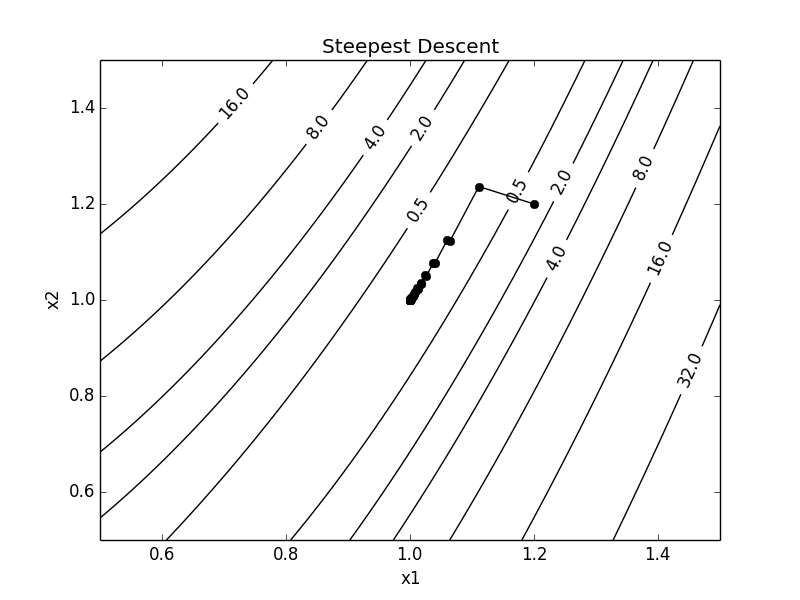
\includegraphics[scale=.5]{Figures/02_1}
    \end{center}

  \item % #6 Done
    Consider the function:
    \[
      f(\v{x}) = 20(x_2 - x_1^2)^2 + (1 - x_1)^2
    \]
    Write a \MATLAB Newton descent code to find the minimizer of this function.
    The function be in the form
    \begin{lstlisting}[language=MATLAB, frame=none]
      xstar = NewtonDescent(f, x0, TOL, MaxIters)
    \end{lstlisting}
    Use $\v{x_0} = (1.2, 1.2)^T$.
    Use $\alpha = 1$.
    Use the backslash operator to invert the appropriate matrices.
    Plot the contour lines of $f$ and superimport the various guesses (each
    connected to the next via a line segment) made by the Newton descent
    algorithm.
    Produce a table of your approximations and the errors (if there are many
    iterations, you can just show the first 10 iterations and the last 10
    iterations).

    The following script implements and runs Newton's Method in multi dimensions
    to find the minimum of $f$.
    Note that this script uses the plotResults function from the script in the
    previous problem.
    \lstinputlisting[language=Python, firstline=28]{02_6.py}
    The following table describes the list of approximations and errors.
    Note that the error at step $k$ is equal to the function value at
    $\p{x_1}_k$ and $\p{x_2}_k$, because the minimum value is zero.
    \begin{center}
      \begin{tabular}{cccc}
        \toprule
        $k$ & $\p{x_1}_k$ & $\p{x_2}_k$ & $e_k$ \\
        \midrule
        0 & 1.2            & 1.2           & 1.1919999999 \\
        1 & 1.181132075471 & 1.39471698113 & 3.2811363464e-02 \\
        2 & 1.002543096882 & 0.97319863783 & 2.0351041753e-02 \\
        3 & 1.001425625865 & 1.00285203539 & 2.0324402951e-06 \\
        4 & 1.000000071205 & 0.99999811020 & 8.2602301879e-11 \\
        5 & 1.000000000005 & 1.00000000001 & 3.3499320311e-23 \\
        \bottomrule
      \end{tabular}
    \end{center}
    The following contour plot was also produced.
    \begin{center}
      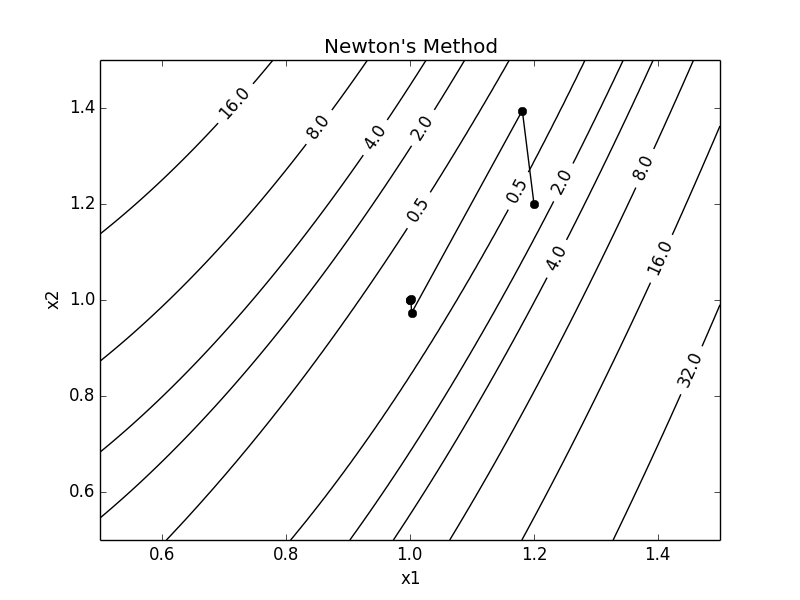
\includegraphics[scale=.5]{Figures/02_2}
    \end{center}

\end{enumerate}
\end{document}
